\documentclass{article}

\usepackage{graphicx}

\begin{document}

\section*{March 15}
Weather: Sunny turning into overcast, followed by a light drizzle and rain past sunset.

Cleared north bed of the pole bean ``mulch'' by placing the ``mulch'' in the compost. Trying to use pole beans to mulch was a \textit{bad} idea, as all it did was create a slug paradise.

Planted the Southern Row of Peas. Used 3 cups of TCF (Territorial's Complete Fetilizer) spread amongst the South Row, but tilled the whole bed. Sowed Peas approximately 1.5 inches deep, attempting ``several seeds per inch'', but probably ended up a bit short.

\begin{figure}
\protect 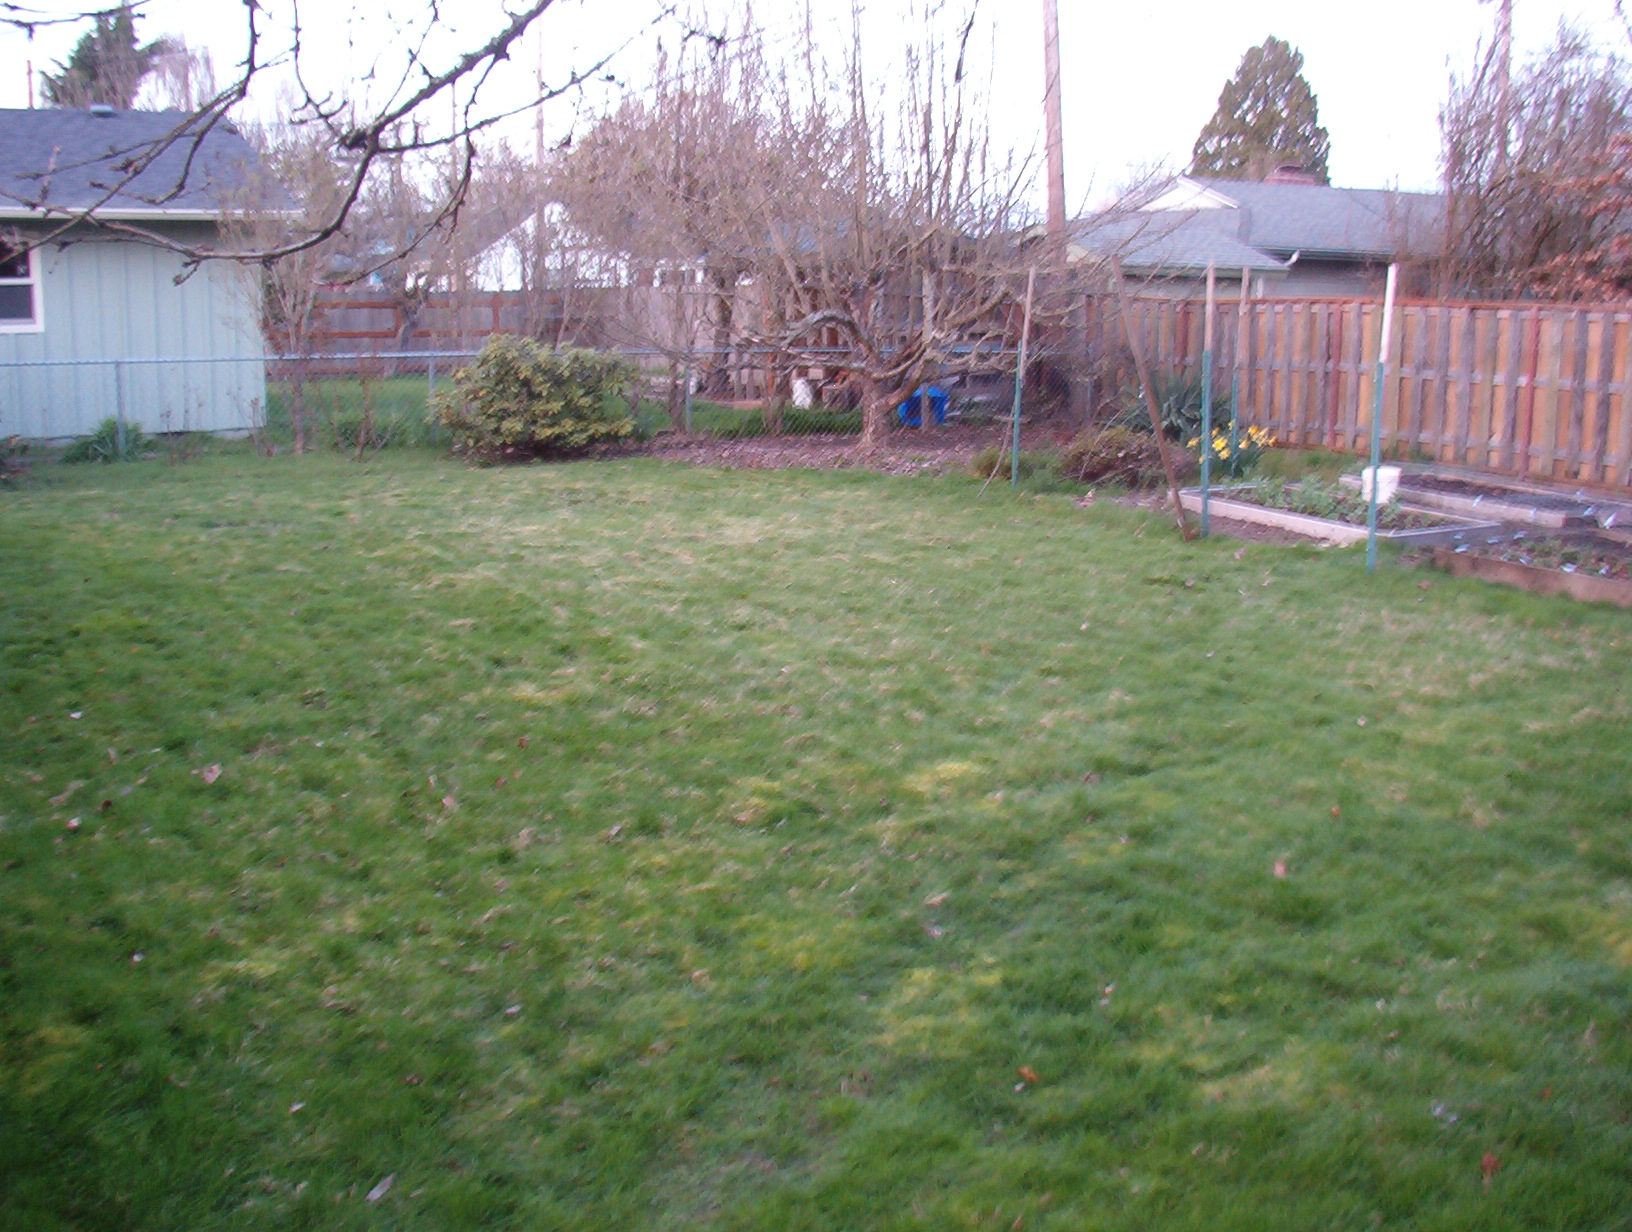
\includegraphics[scale=0.20]{pics/0315_garden1.jpg}
\caption{Weekly north-facing picture of the garden.}
\end{figure}
\begin{figure}
\protect 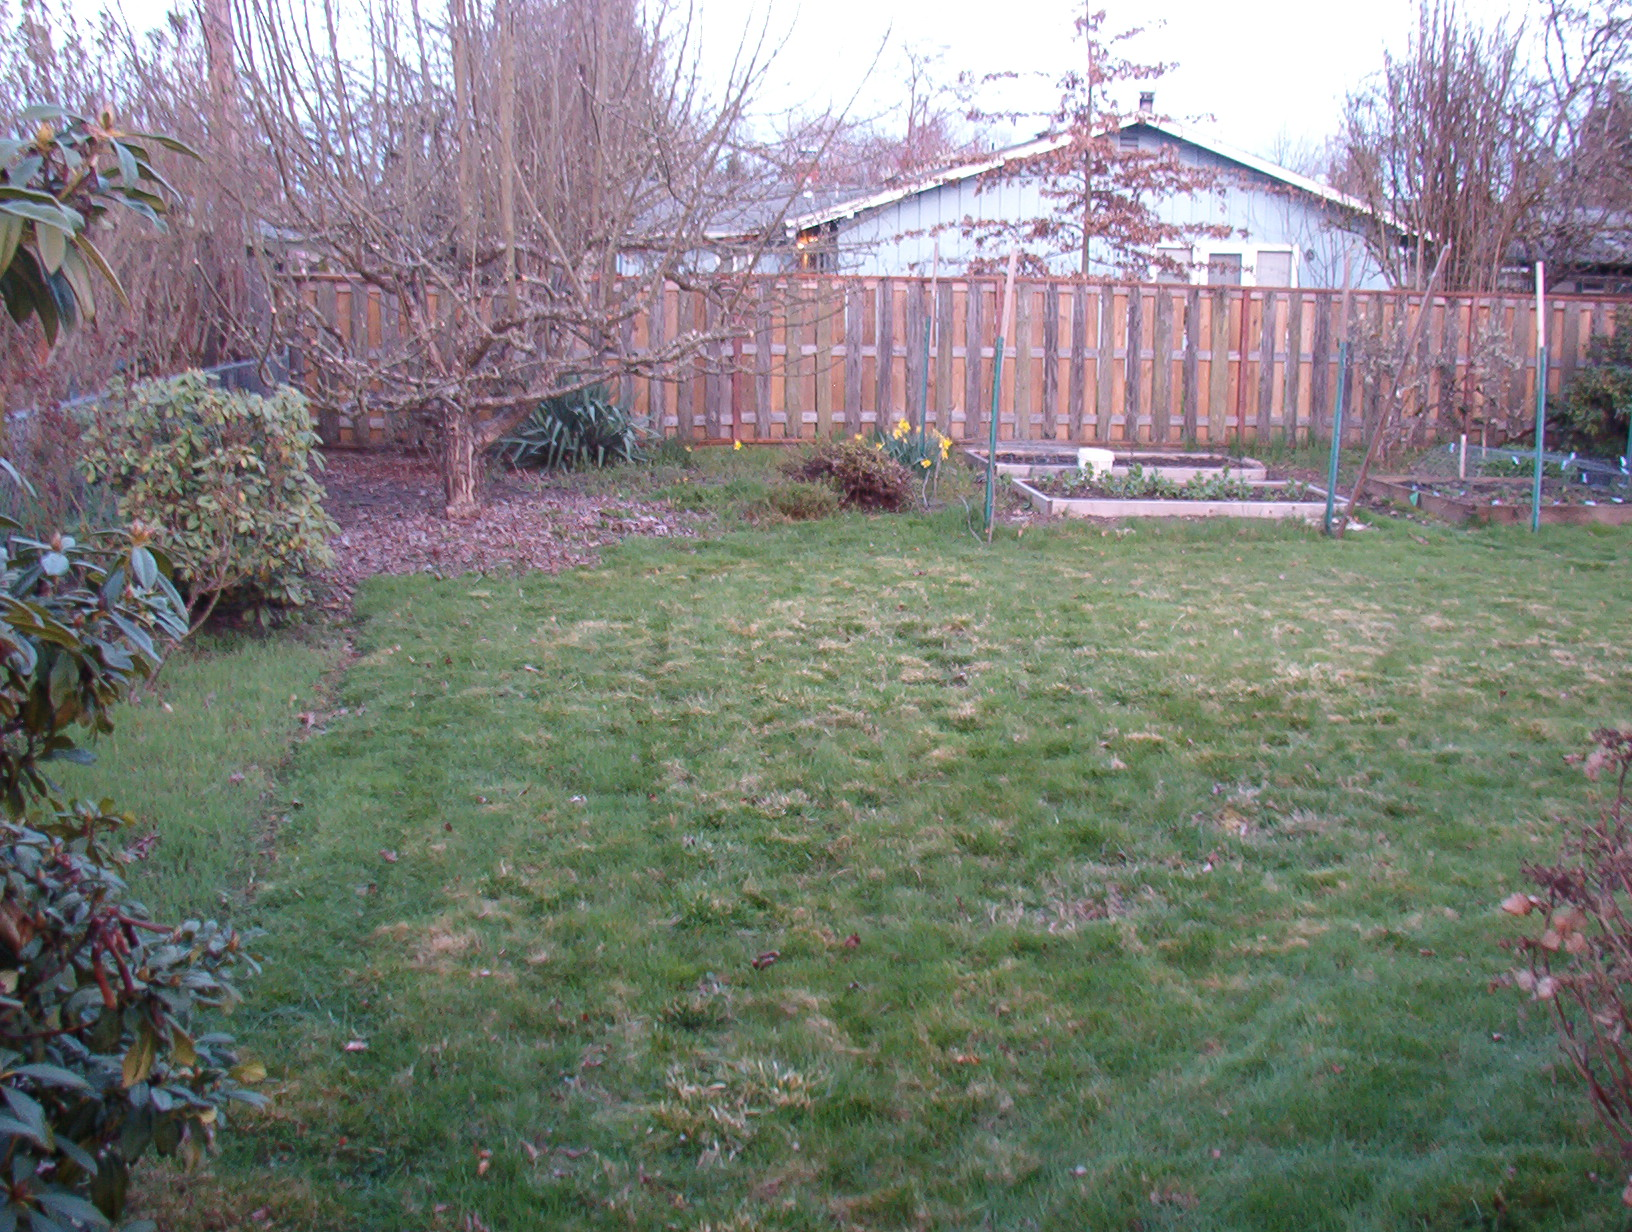
\includegraphics[scale=0.20]{pics/0315_garden2.jpg}
\caption{Weekly east-facing picture of the garden.}
\end{figure}

\section*{March 16}
Weather: Overcast, windy, and cold. Very ominous.

Found issue with garden plan that added extra foot to the available area; managed to fix by compressing the path up against the bed (I wasn't planning on walking that path anyways, right?).

Placed posts to showing started and ending locations of each vegetable patch, except for the one next to the raised bed, since a bush in the way of the final ending point.

\section*{March 17}
Weather: Sunny with a few clouds.

Prepared the Spinach bed. Since the area was already covered by grass, I shoveled the grass off to one side then dug a bit deeper and shoveled the deeper subsoil to another side; I then put the grass back into the bed followed by the deeper subsoil; this may or may not work, because the top and subsoil are horrendous clay. I then tilled 2 cups of TCF into the top 6 row-feet of the bed and attempted to plant about 3 seeds per inch, but probably planted quite a bit more than that (see Figure \ref{0317sowingspinach}) \\
\begin{figure}
\protect 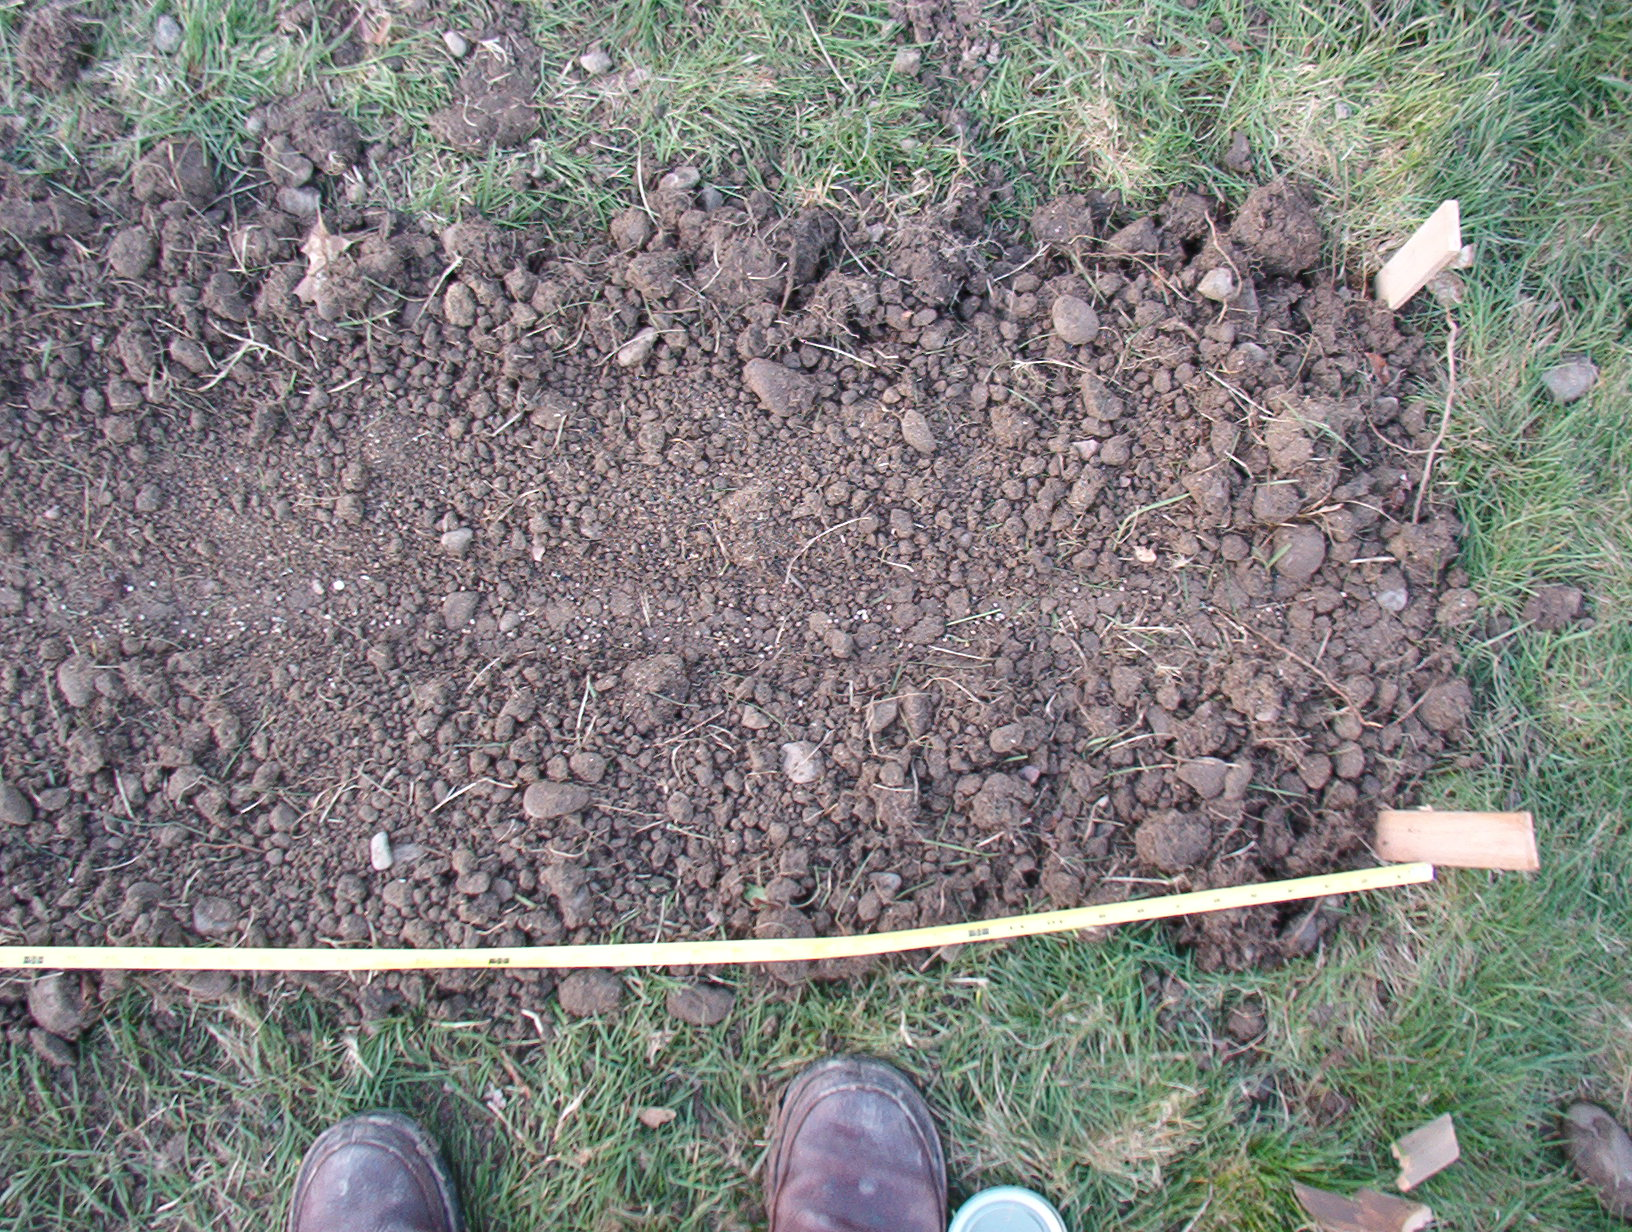
\includegraphics[scale=0.20]{pics/0317_spinach1.jpg}
\protect 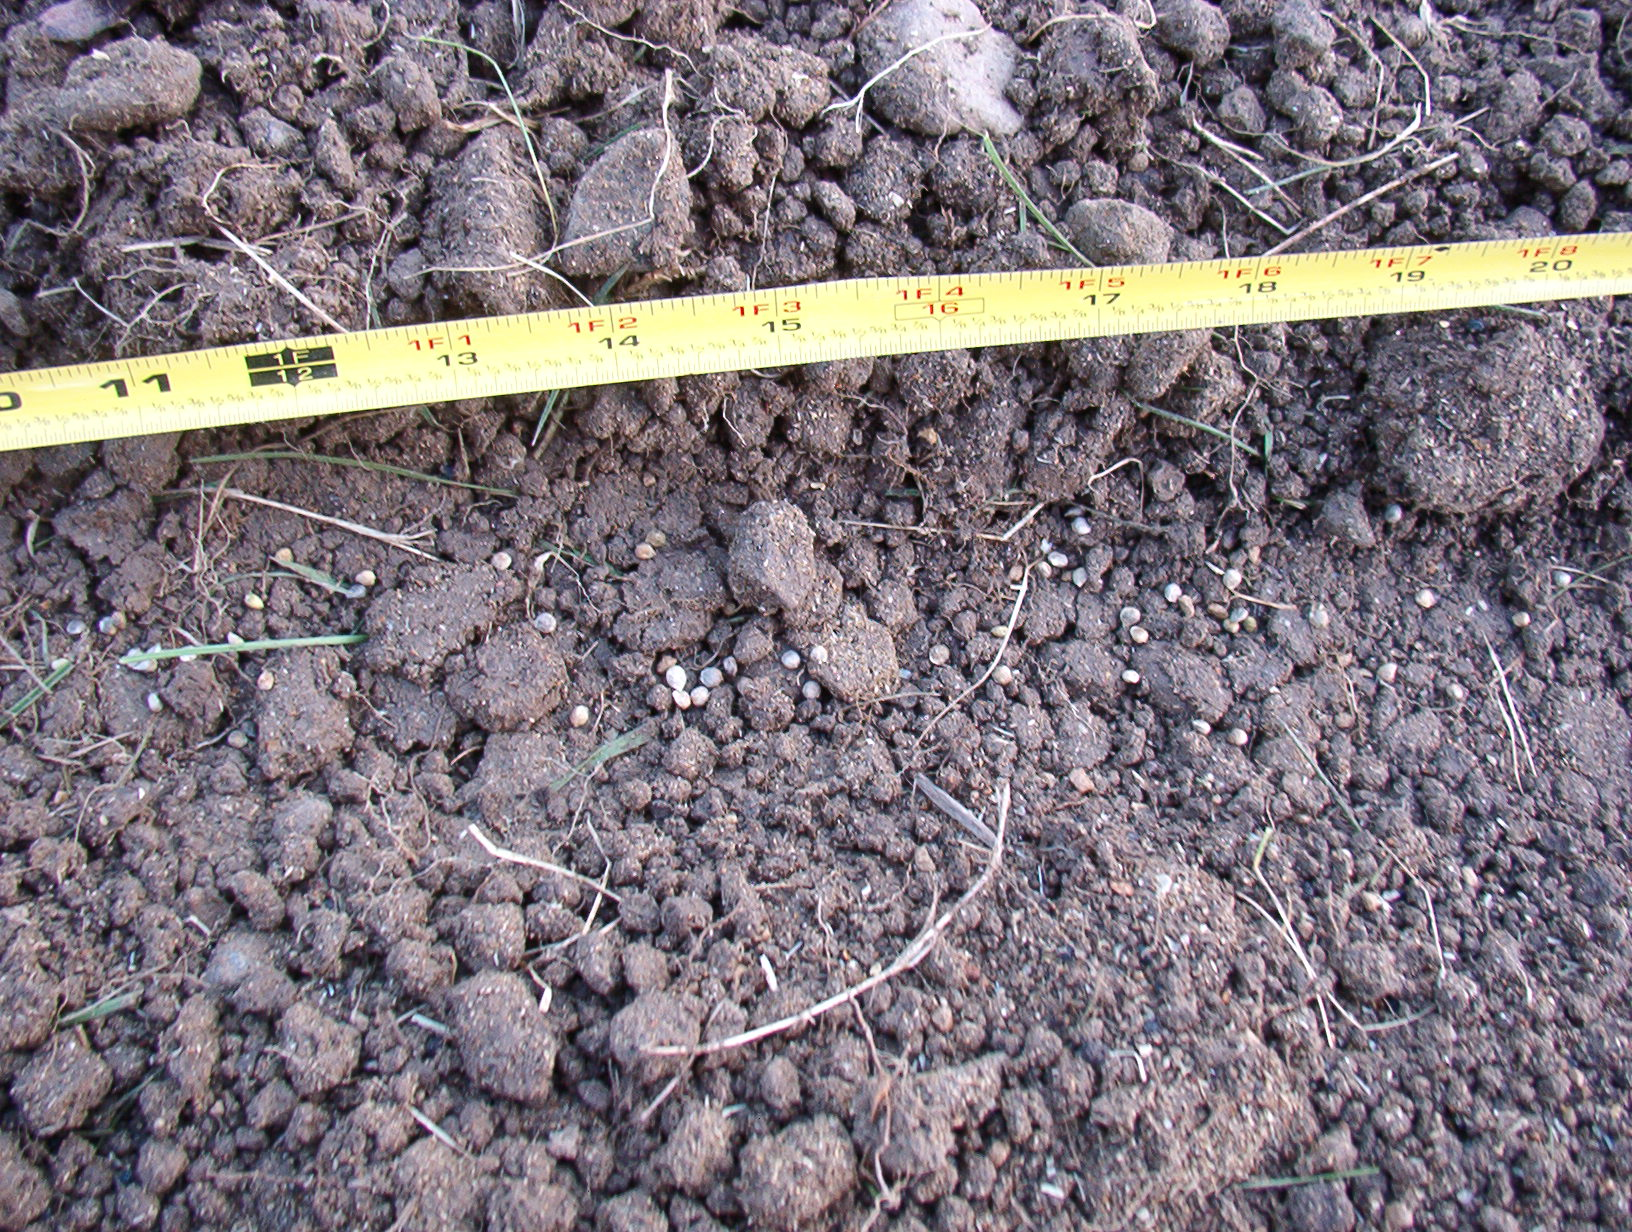
\includegraphics[scale=0.20]{pics/0317_spinach2.jpg}
\caption{Sowing spinach seeds.}
\label{0317sowingspinach}
\end{figure}
That should be okay, since I expect heavy losses. I also expect to side-dress abundantly once (perhaps ``if'') the Spinach germinates. Sown approximately 0.5 inches deep. May need to buy more Spinach needs. I'd like to cover the grass around the bed with paper in order to kill the grass, too, before it starts trying to take over the bed. \\
\begin{figure}
\protect 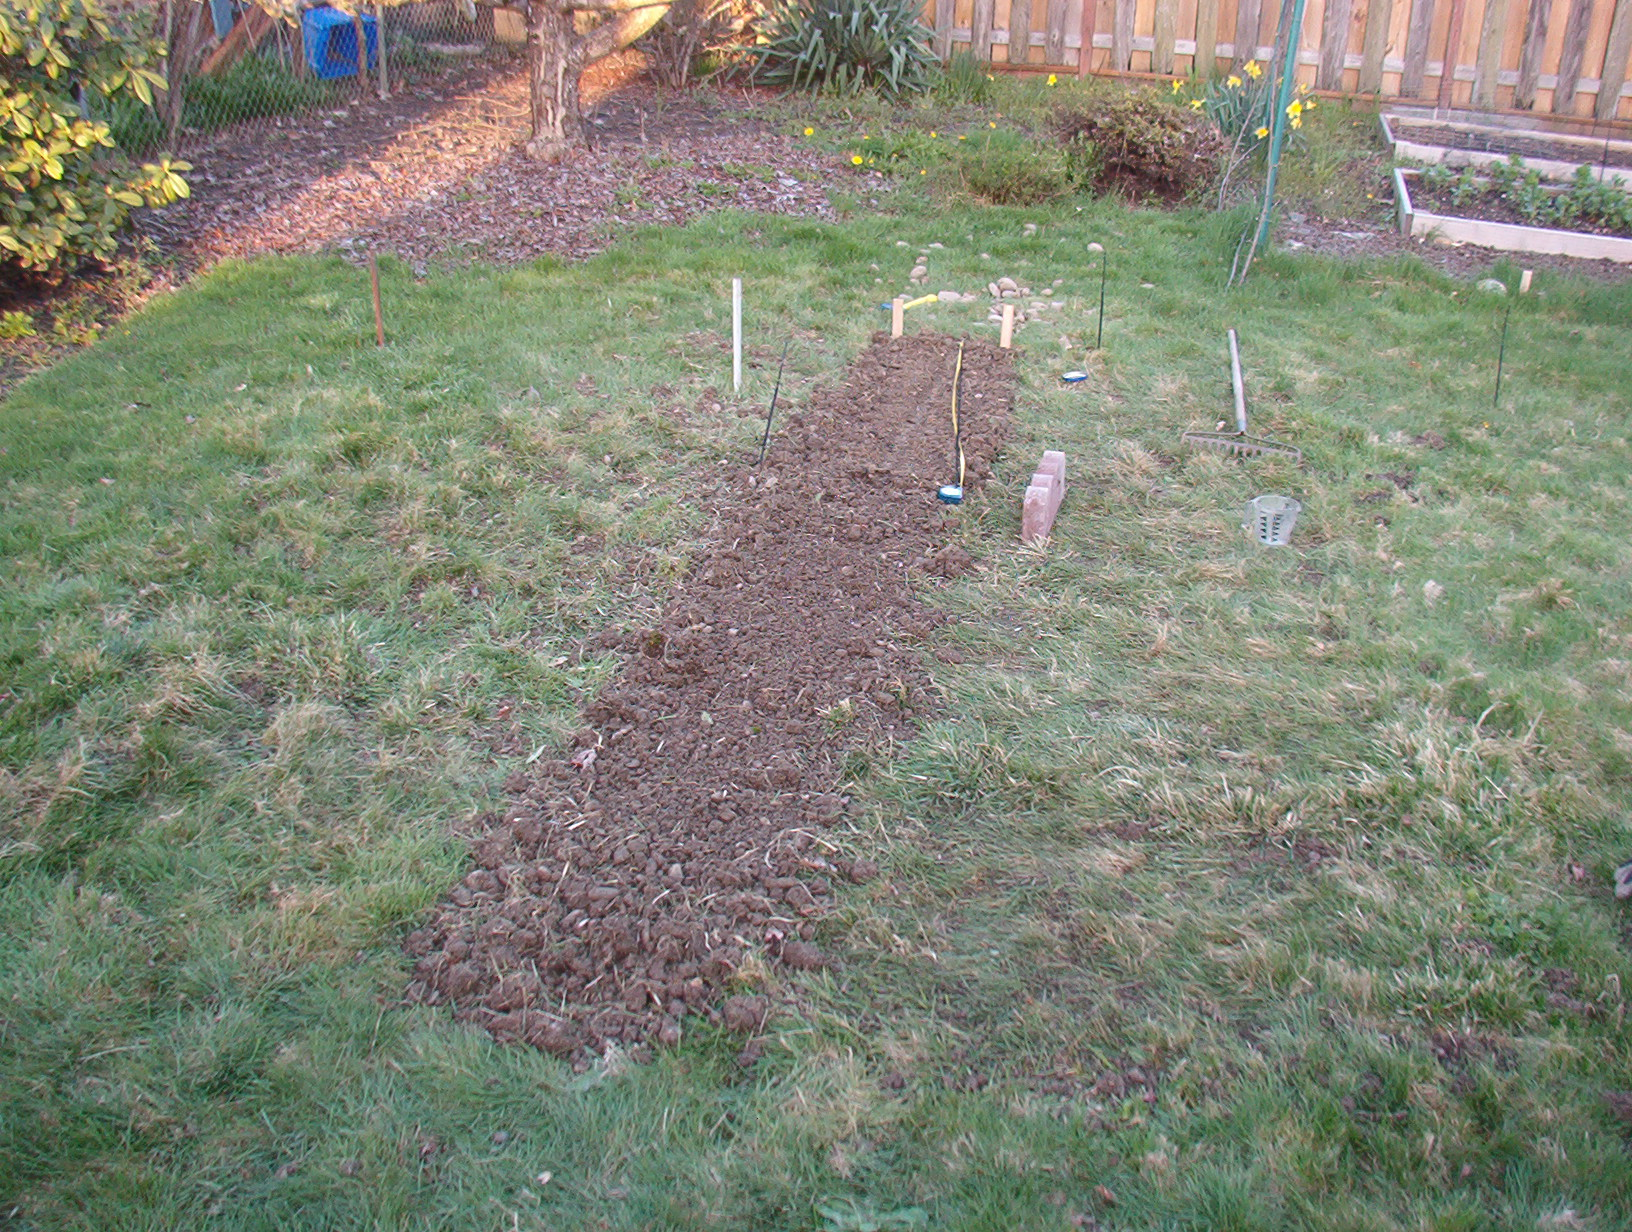
\includegraphics[scale=0.20]{pics/0317_bed.jpg}
\caption{Spinach bed after sowing.}
\end{figure}

\section*{March 18}
Weather: Sunny with a slightly cold breeze.

Started onion transplants. Using 50-cell container with spherical cells slightly less than 2 inches in diameter. For soil, used a slightly modified version of Solomon's Potting Mix as I did not have any compost ready; used 24 cups of garden soil from the raised bed (which the onions will be transplanted into), 8 cups of pre-moistened spaghum moss, $\frac{3}{4}$ cups of TCF, and around $\frac{1}{10}$ cup of agricultural lime. The seed packet had about half as many seeds as I would have liked, but I planted about 3 seeds in 6 rows and 2 seeds in the remaining 4 rows. Planted approximately $\frac{1}{2}$ an inch deep. I'm going to leave the container in my room... hopefully that environment works for them.
\begin{figure}
\protect 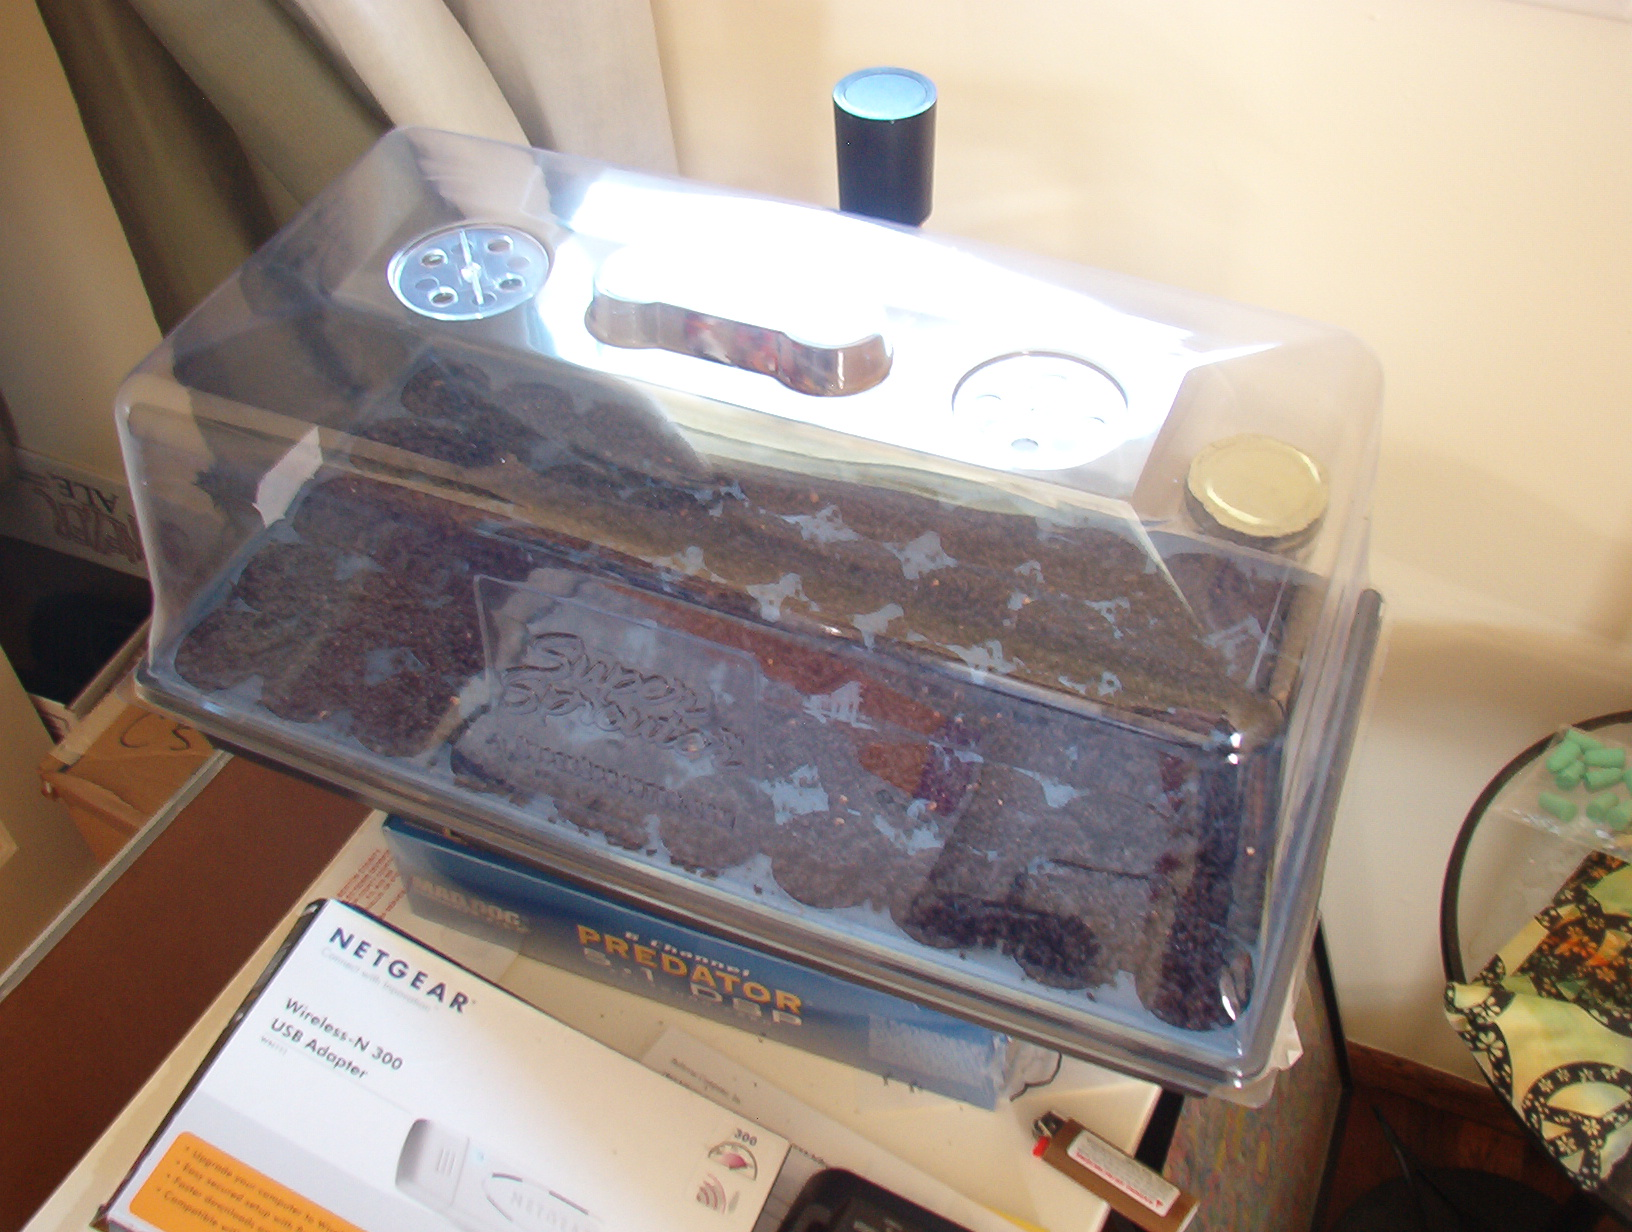
\includegraphics[scale=0.20]{pics/0318_onions.jpg}
\caption{Onion transplants.}
\end{figure}

The Spinach bed soil looks like something suitable for the Mars Rover competition; completely dry and lifeless. I've started a basic soil-composition test that needs to sit for a few days in order to see what might improve the soil's tilth. I've also covered the area near the Spinach with Newspapers to start killing off the grass so it doesn't take over and eat any of the added fetilizer; the Newspaper was weighed down using rocks that were dug up from the subsoil.
\begin{figure}
\protect 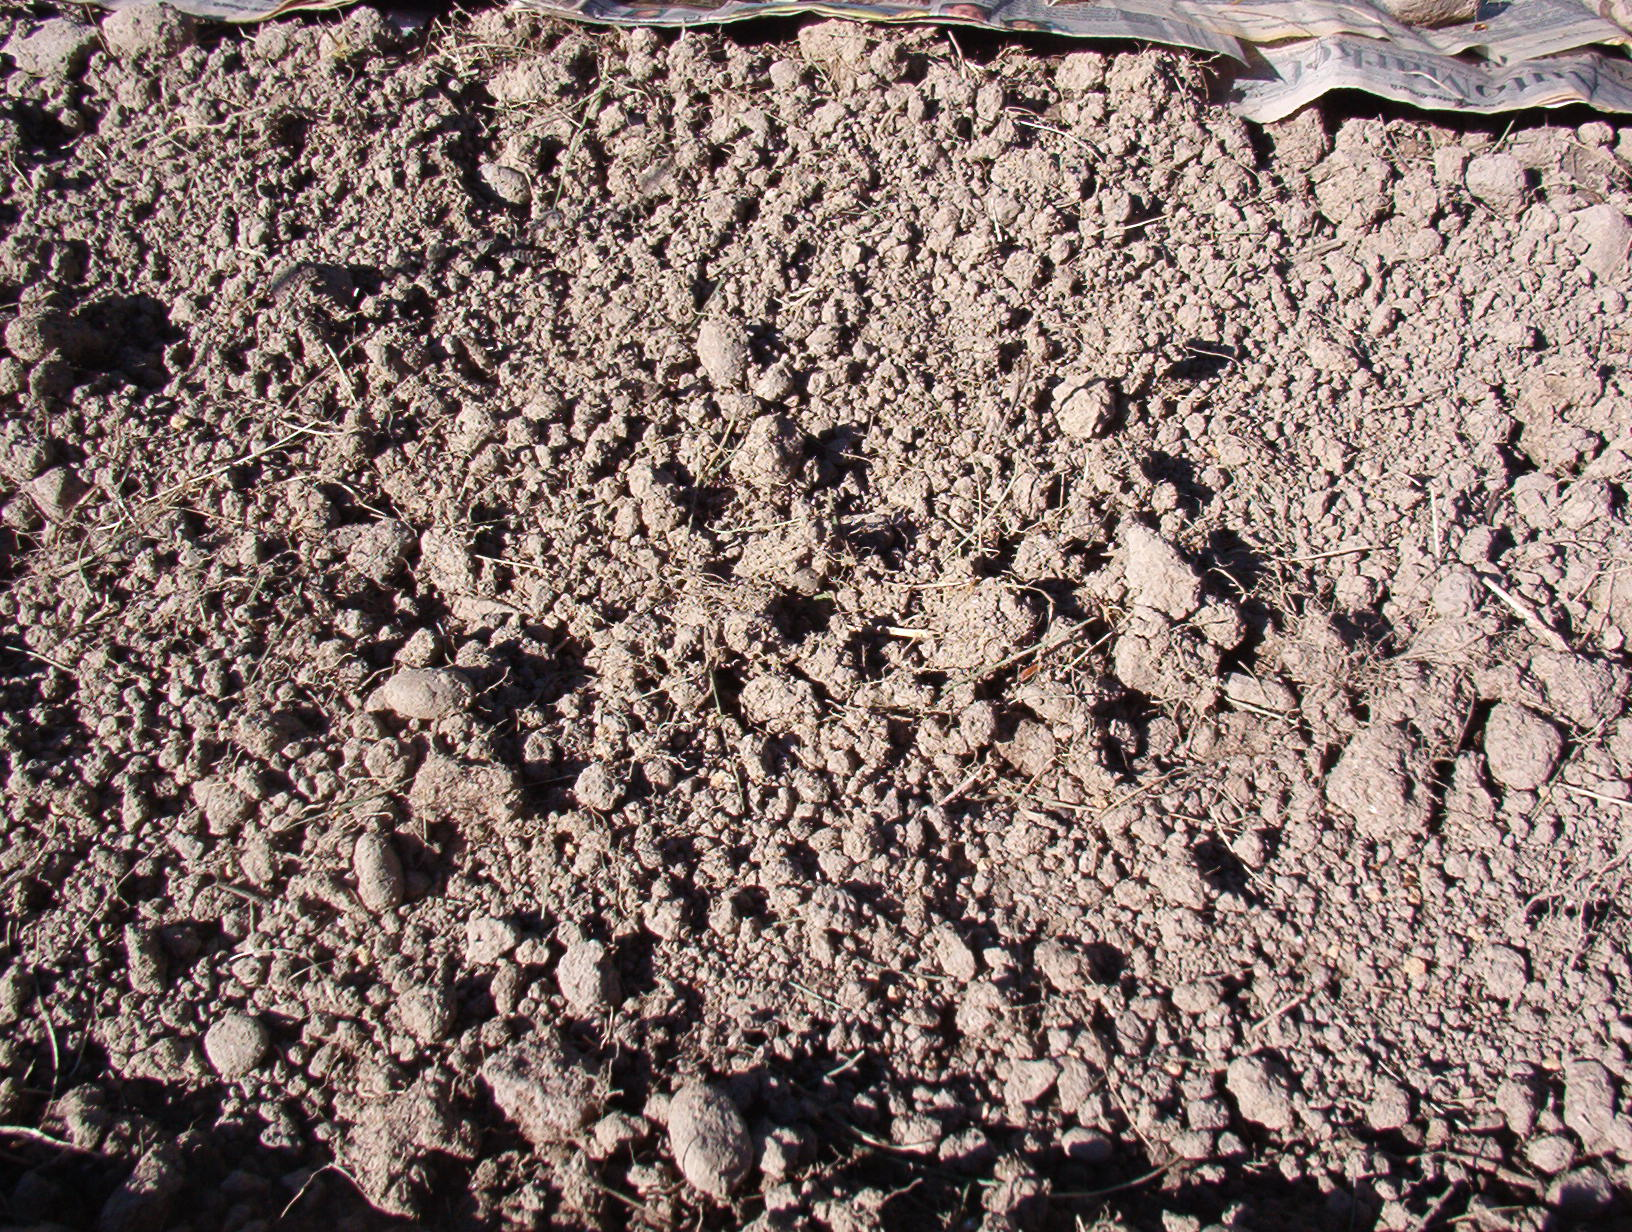
\includegraphics[scale=0.20]{pics/0318_spinach2.jpg}
\caption{Spinach soil vaguely resembles the surface of Mars.}
\end{figure}
\begin{figure}
\protect 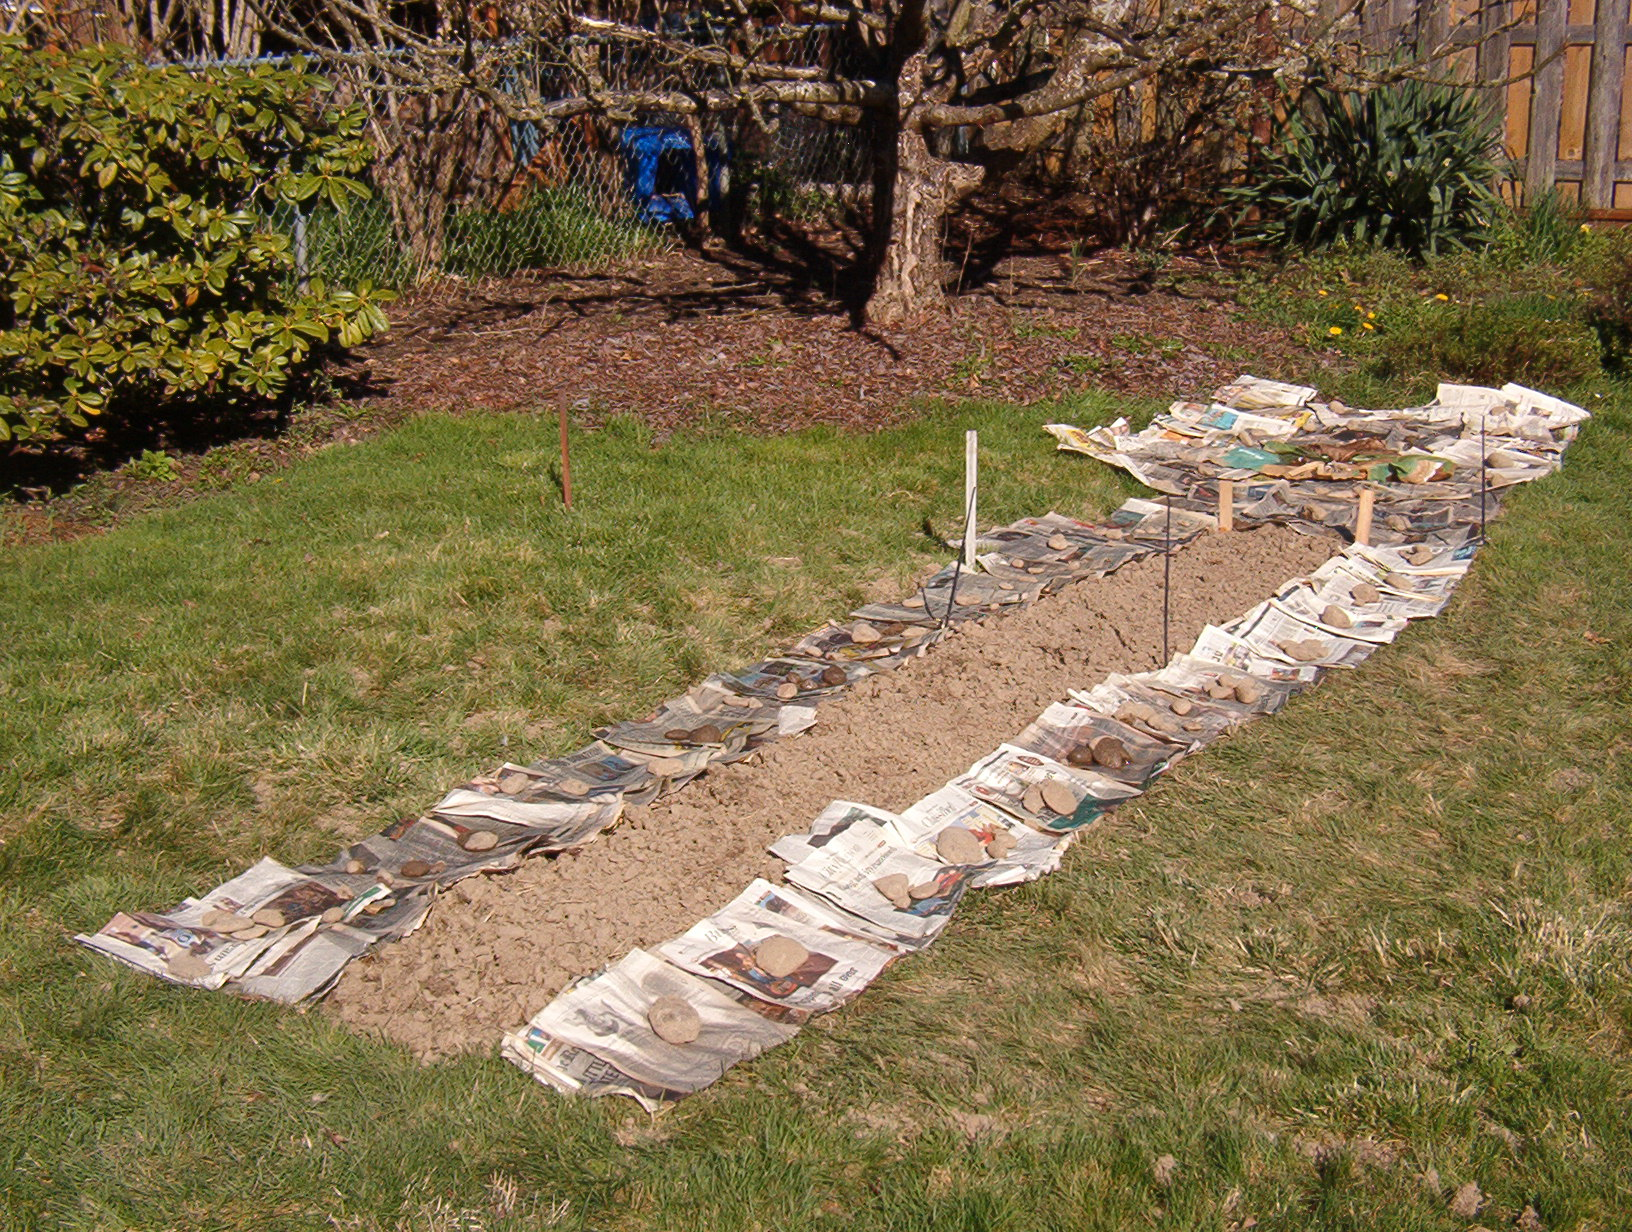
\includegraphics[scale=0.20]{pics/0318_spinach1.jpg}
\caption{Spinach bed surrounded by Newspaper.}
\end{figure}

Also, I found it mildly irksome that, based on the number of row-feet and seeds-to-sow-per-inch, I knew \textit{how many} seeds I needed, but not the \textit{weight} of seeds that I needed (though this probably depends somewhat on variety, the seeds packets that I picked up from Territorial generally did not have an approximate count). So, I took the time to count the seeds I got in each packet. The results are:
\begin{itemize}
	\item Onion, Cortland: 125 seeds (though I planeted 139 seeds, so apparently counting seeds is hard) in a $\frac{1}{2}$ gram package.
	\item Peas, Oreogn Sugar Pod II: 398 seeds in a 3 ounce package.
	\item Spinach, Space Hybrid: 527 seeds in a 5 gram package.
\end{itemize}

\section*{March 19}
Weather: Partly cloudy.

\section*{March 20}
Weather: Partly cloudy, cold temperature outside.

Began digging up beet patch.

\section*{March 21}
Weather: Sunny and mildly cold out.

Finished digging beet patch and surrounding it with newspaper. Began digging North potato patch. Watered seedlings. Soil test inconclusive; will need a bright light or something in order to see sand/clay levels accurately.
\end{document}

\section*{March 22}
Weather: Sunny and mildly cold out.

Continuted digging North potato patch.
\begin{figure}
\protect 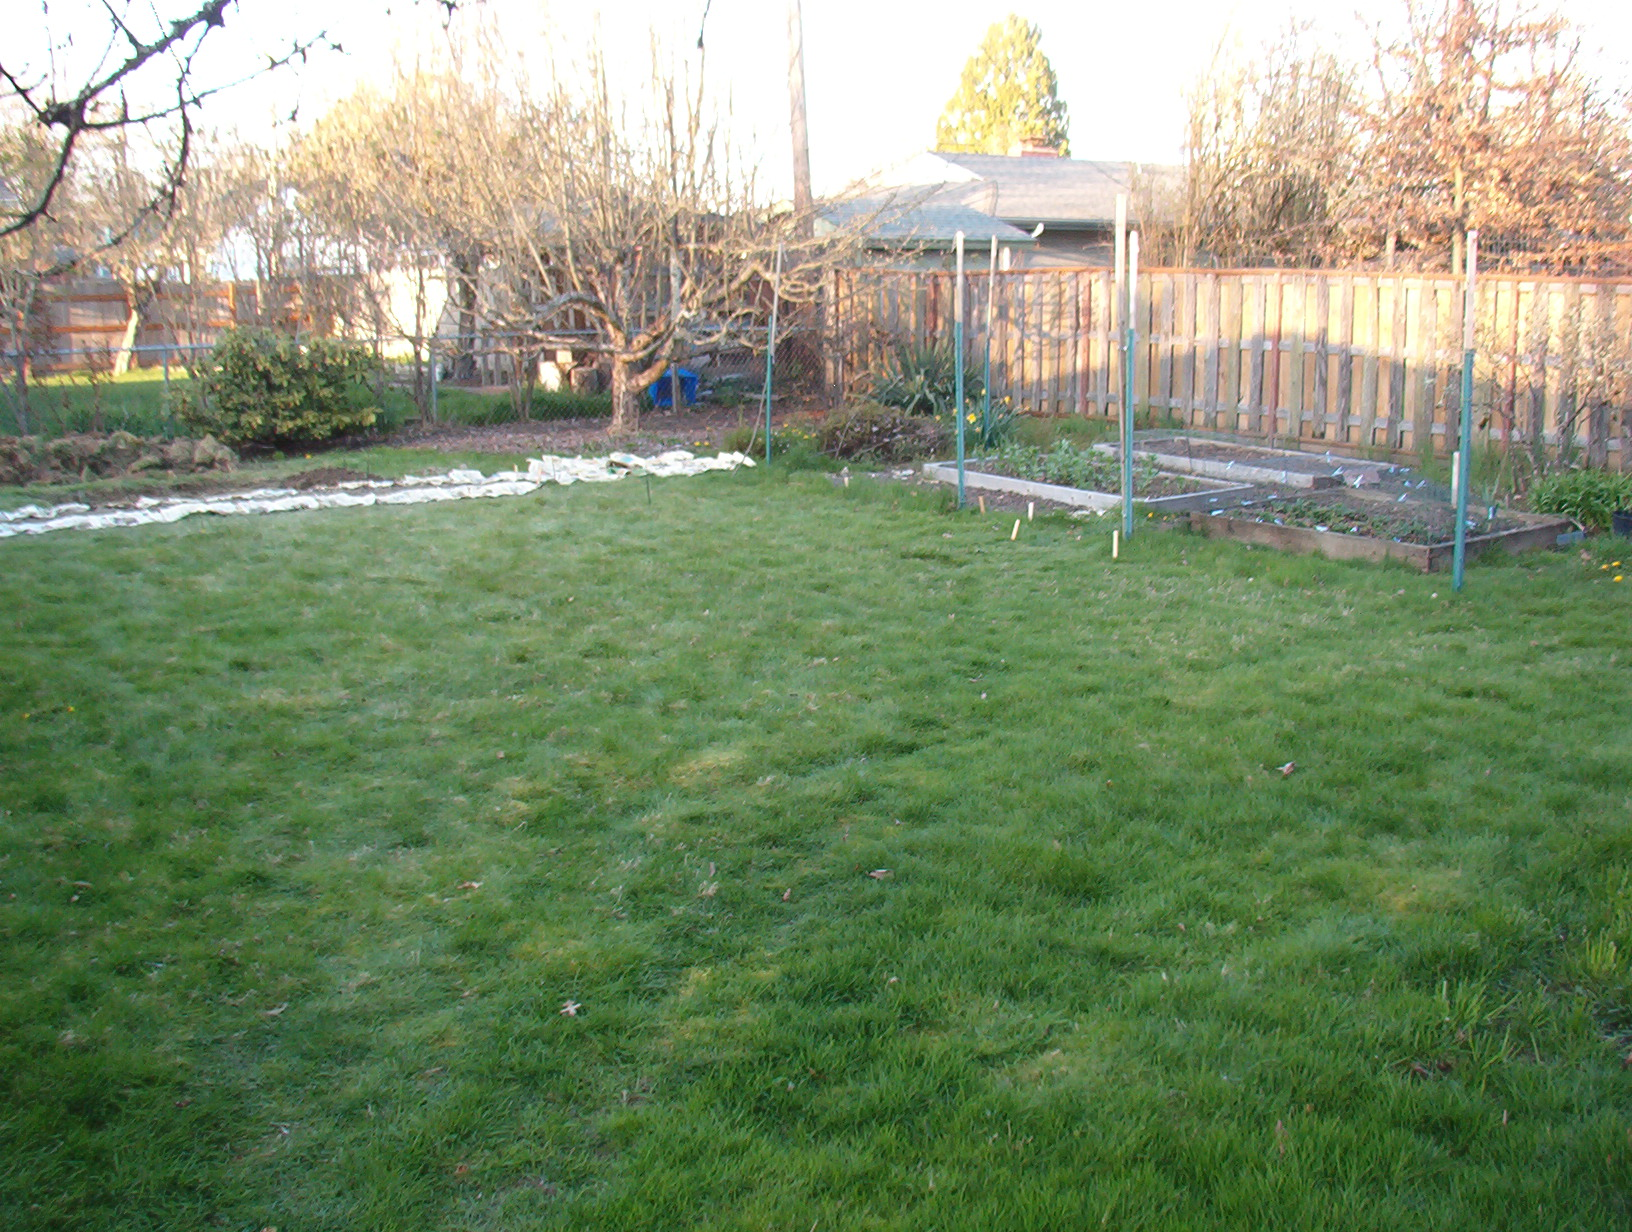
\includegraphics[scale=0.20]{pics/0322_garden1.jpg}
\caption Weekly North-facing picture of the garden.
\end{figure}
\begin{figure}
\protect 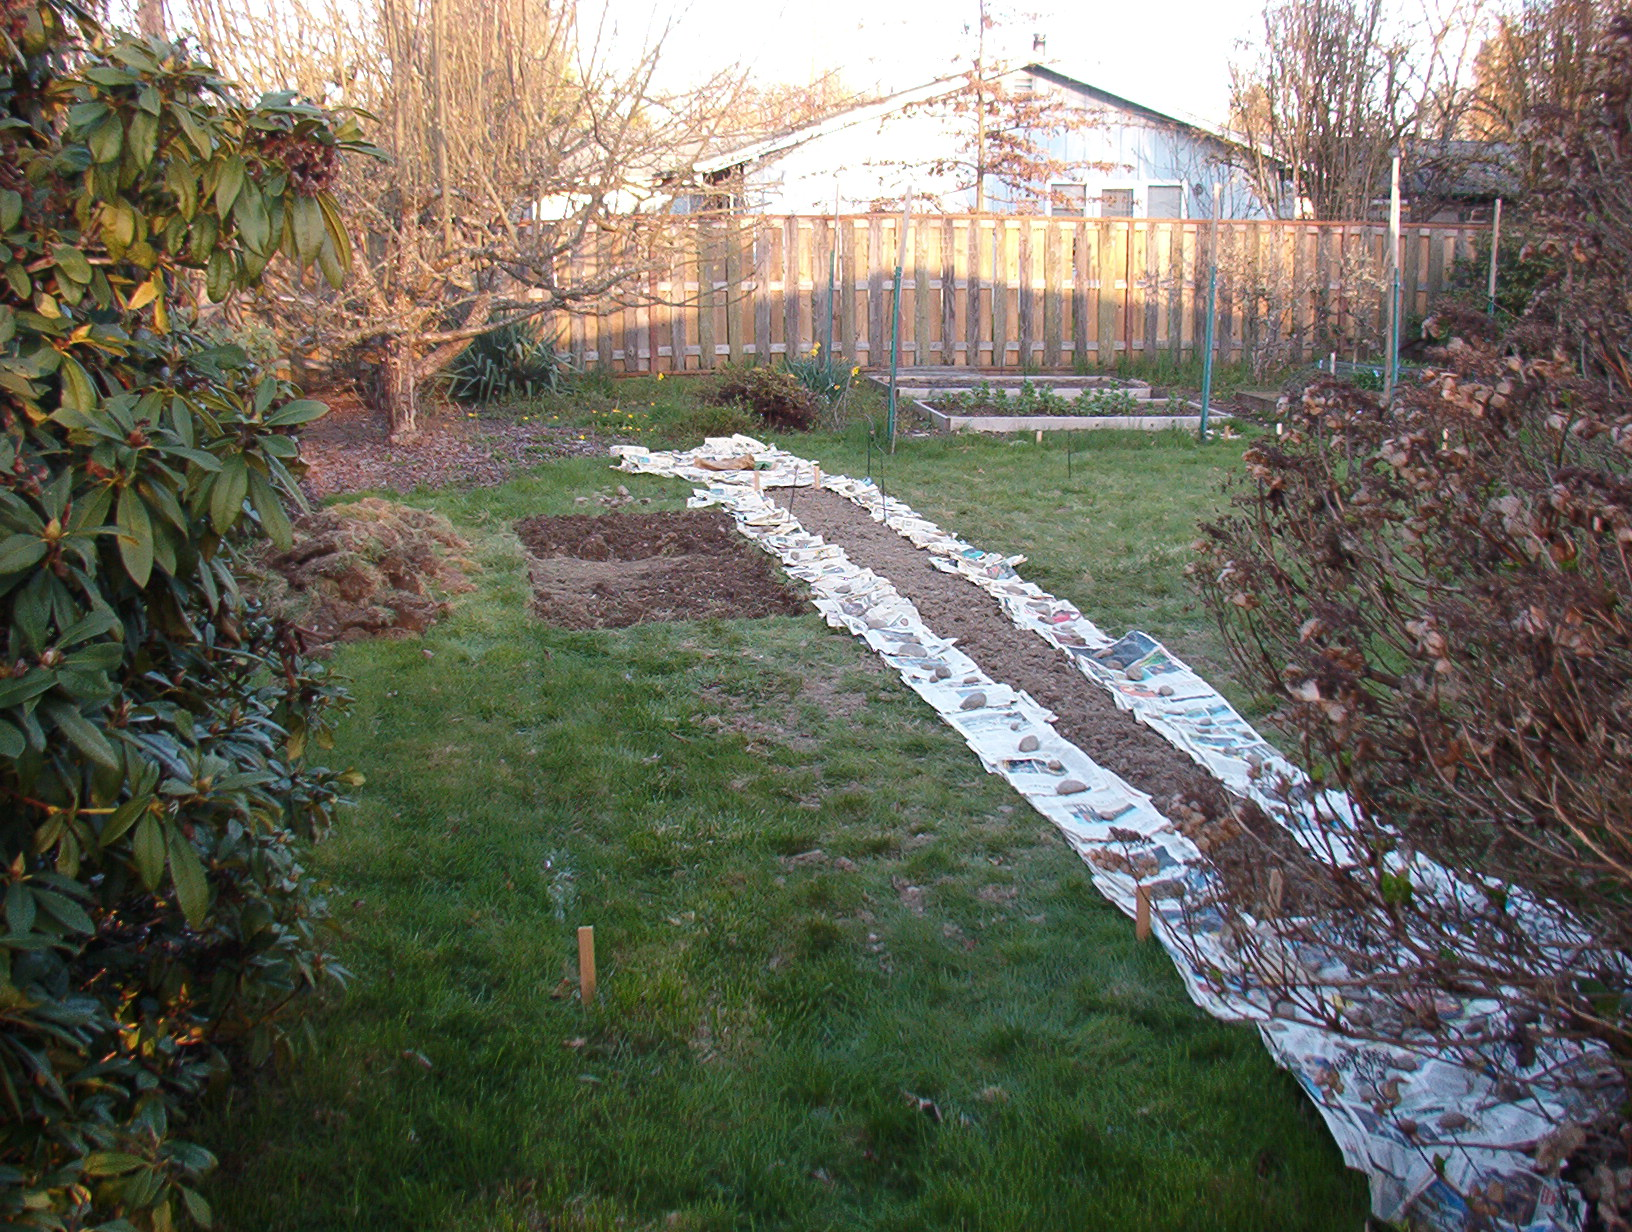
\includegraphics[scale=0.20]{pics/0322_garden2.jpg}
\caption{Weekly East-facing picture of the garden.}
\end{figure}
